\section{Drag Force and Terminal Velocity}

\instructornote{%
By Matt Trawick, Fall 2019.  Time: 40-50 minutes.

Students don't all get beautiful results for the power law.  Encourage them to take careful data; multiple tries (and multiple values for $v_T$) would help, of course.  
Difficulties aside, I (Matt) think this lab is good enough that I plan to use it again.  

Additional note by Matt: I did not cover this topic along with the chapters on Newton's laws.  I waited and did this topic (and this lab) much later in the semester, after I had already done work and energy.  This way, once I introduced the idea of drag, I could immediately assign problems like ``how much power does a truck's engine need to have in order to maintain a steady speed of 70 mph.''
}

\makelabheader %(Space for student name, etc., defined in master.tex or labmanual_formatting_commands.tex)

\bigskip
\textbf{Apparatus}

\begin{itemize}[nosep]
\item \textit{Capstone} software (\filename{P\_V\_A\_Sensor\_Graphs.cap} experiment file)
\item Coffee filters (x5)
\item High precision digital lab scale
\item Ruler
\item Wireless motion sensor (mounted high on lab stand, pointed down)
\end{itemize}

\bigskip
\textbf{Activity 1: Predictions and First Data}

A ``drag force'' $F_{\rm drag}$ is a force caused by the air hitting against a moving object.  You would feel a drag force if you held your arm out of a moving car, for instance.\footnote{Don't try this at home.  Keep arms and legs inside moving vehicle at all times.}
  
\begin{enumerate}[labparts]
\item If the car's speed increased, would the drag force on your hand increase, decrease, or stay the same?
\answerspace{0.3in}

\item Suppose you drop an object, like a ball or a tissue.  Draw a free body diagram for the object as it falls, including the drag force.
\answerspace{1.2in}

\item Are the two forces in your diagram always constant during the fall?  Or will either of them change over time?  (Hint: does the object fall with constant speed?)
\answerspace{0.5in}

\item Would the falling object continue to accelerate if the drag force and the gravitational force were equal?
\answerspace{0.5in}

\item On the axes below, draw a sketch with a dashed line predicting the shape of the velocity vs. time graph for a falling object (such as a ball or a tissue), including the effect of a drag force.  Assume the falling object starts from rest, $v=0$.

\begin{lab_axis}*[lab_noticks_1quad,
	height = {1.2in}, width = {3.0in},
	xlabel={Time},
	ylabel={Velocity},
	]
\end{lab_axis}

\item Now let's do the experiment.  Open the file \filename{P\_V\_A\_Sensor\_Graphs.cap}, located in the \filename{\coursefolder} folder. Turn on the motion sensor at your station and connect it to the computer via Bluetooth. Use a stack of three coffee filters nested inside each other, dropping them from just below the sensor to obtain a graph of $v(t)$.  You may need to try this a few times to get a smooth graph.  If your stack of filters flutters side to side, try bending the edges up to make the filters less flat.  Once you have a good velocity graph, sketch its shape with a solid line on the axes below.  

\begin{lab_axis}*[lab_grid,
	xlabel={Time (s)},
	ylabel={Velocity (m/s)},
	width=4.5in, height=1.8in,
	xmin=0, xmax=5,
	ymin=-2, ymax=2,
	xtick distance = 1,
%	ytick distance = 1,
	minor x tick num=1,
%	minor y tick num=1,
	]
\end{lab_axis}

\item Indicate on your graph the place where $F_{\rm drag} = F_{\rm grav}$.  

\item The maximum speed of the falling object, reached when $F_{\rm drag} = F_{\rm grav}$ is called the ``terminal velocity'' $v_T$.  What is $v_T$ for your stack of three coffee filters?
\answerspace{0.5in}

\end{enumerate}

\medskip
\textbf{Activity 2: Drag Force \textit{vs.}~Velocity}

%You found in the previous activity that the maximum speed, or ``terminal velocity'' $v_T$ 
%is reached when  $F_{\rm drag} = F_{\rm grav}$.  
In this activity, you will measure 
$F_{\rm drag}$ as a function of velocity $v$ by recording the terminal velocity $v_T$ for stacks of filters with different weights.

\begin{enumerate}[labparts]
\item Measure the terminal velocity $v_T$ for a single coffee filter, and also for nested stacks of up to five coffee filters.  
Try to make sure the shape of each falling stack is always the same; bend the edges up or down as needed.
Record your results in the table below.

\begin{center}
{\renewcommand{\arraystretch}{1.8}
\begin{tabular}{|c | c| C{1in} |}
\hline
$n$ & $F_{\rm drag}~ (= F_{\rm grav}$) at $v_T$ & $v_T$ \\ 
\hhline{|=|=|=|}
1 & & \\ \hline
2 & & \\ \hline
3 & & \\ \hline
4 & & \\ \hline
5 & & \\ \hline
\end{tabular}
}
\end{center}

\pagebreak[2]
\item Copy your data from the table above into \textit{Excel}.  Make a graph of $F_{\rm drag}$ \textit{vs.}~$v_T$, plotting the force on the $y$~axis and the speed on the $x$~axis.
Note the twist here: your goal is to understand how the drag force $F_{\rm drag}(v)$ varies as a function of speed $v$.
This is conceptually the reverse of the experiment you did, where the force was more like the \textit{independent} variable (which you set by changing $F_{\rm grav}$, by altering the number of filters) and the terminal velocity was more like the \textit{dependent} variable which you measured as a result.

\item For very low speeds, or for objects moving in incompressible fluids like water, the drag force is typically proportional to $v$.  In many other cases, the drag force is often proportional to $v^2$.  Does your data suggest a power law relationship $F_{\rm drag} \propto v^p$?  Use a fit to determine what exponent $p$ is most consistent with your data.  Write your value of $p$ below, and also print a copy of your graph if your instructor requests it.
\answerspace{0.8in}

For objects in air at moderate speeds, the drag force on an object can be expressed as
\begin{equation}
F_{\rm drag} = \frac{1}{2}C \rho A v^2,
\end{equation}
where $\rho$ is the density of air (1.2~kg/m$^3$ at room temperature and atmospheric pressure), 
$A$ is the object's cross-sectional area, and 
$C$ is a dimensionless ``drag coefficient'' based on the object's shape.  
You can think of $C$ as a measure of how ``aerodynamic'' an object is.  The table below shows a few examples.

\begin{center}
{\renewcommand{\arraystretch}{1.2}
\begin{tabular}{|c | c |}
\hline
object & drag coefficient $C$ \\ 
\hhline{|=|=|}
sphere & 0.47 \\ \hline
cube & 1.05 \\ \hline
Toyota Prius & 0.25 \\ \hline
typical pickup truck & 0.40 \\ \hline
\end{tabular}
}
\end{center}

\item What is the cross-sectional area $A$ of your stack of coffee filters?  Note that this is NOT the actual surface area of the filters.  It's more like the area of the \textit{shadow} cast by the filters if light were shining in the direction of motion.
\answerspace{0.8in}

%\hspace{\fill}
%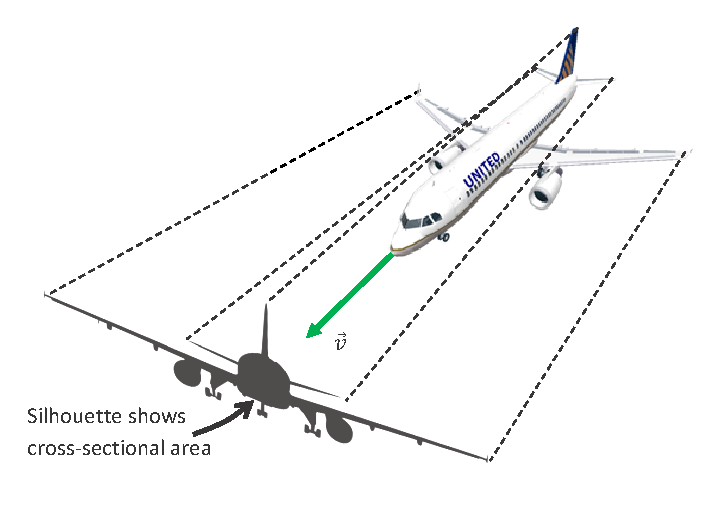
\includegraphics[scale=0.8]{drag_force/cross_sectional_area.eps}

Next, you will perform a fit of your data to Equation (1) above.  To do this, you will use the LINEST function in \textit{Excel}, described in \textbf{Appendix \ref{excel}}.  But to make LINEST fit your $F_{\rm drag}$ values to $v^2$ instead of $v$, you will enter ``\specialcaret \verb!2!'' after selecting your $v$ data (what \textit{Excel} calls the ``known $x$ values'') so that your entire line will look something like ``\verb!=linest(B1:B5, A1:A5!\specialcaret \verb!2, 0, 1)!''.
\item Based on your data, what is the drag coefficient $C$ for your stack of coffee filters?  Also check that your number seems sensible in light of the other values of $C$ in the table above.  Is your stack of coffee filters as ``aerodynamic'' as a Toyota Prius?
\answerspace{0.8in}


\end{enumerate}

